% REACH -- AISTATS 2027 submission (official aistats2027.sty; anonymous by default).
%
% ANONYMISATION (check before upload):
%   - no author names, affiliations, acknowledgements, grant numbers, or repo/Modal URLs
%   - cite own prior work in the third person
%   - strip PDF metadata and figure metadata; supplementary code without user paths or app names
\documentclass[twoside]{article}
\usepackage{aistats2027}
\usepackage[utf8]{inputenc}
\usepackage[T1]{fontenc}
\usepackage{amsmath,amssymb,amsthm,booktabs,graphicx,natbib,xcolor,amsfonts}
\usepackage[hidelinks]{hyperref}
\usepackage[capitalise,noabbrev]{cleveref}
\hypersetup{pdfauthor={},pdftitle={}}

\newcommand{\Wcls}{\ensuremath{W_{\mathrm{cls}}}}
\newcommand{\Wlab}{\ensuremath{W_{\mathrm{label}}}}
\newcommand{\Wunk}{\ensuremath{W_{\mathrm{unk}}}}
\newtheorem{proposition}{Proposition}
\newtheorem{lemma}{Lemma}

\begin{document}
\twocolumn[
\aistatstitle{Which Data Would Reduce This Uncertainty?\\ Acquisition-Attributed Epistemic Widths for Frozen Classifiers}
\aistatsauthor{Anonymous Authors}
\aistatsaddress{Anonymous Institution}]

\begin{abstract}
% Frozen abstract (lock doc), verbatim except "an estimate per-input answer" -> "an estimated
% per-input answer" (author-approved rewording that keeps the hedge).
Epistemic uncertainty is uncertainty that more data can reduce, but which data? For a frozen
classifier with a labeled reference set and additional unlabeled examples, we provide an estimated
per-input answer. From the log we form a maximum mean discrepancy ball of input densities that the log cannot
exclude, spanning prevalence mixtures of the known classes plus a slot for an unseen class. The
spread of the induced label posteriors defines three epistemic widths: prevalence, label and
coverage, each tied to a different acquisition. Under frozen class-conditionals, we characterize
how class distinguishability and support determine when more logging narrows the prevalence and
coverage widths, while the label width, fixed by the labeled reference, remains unchanged. In
controlled synthetic experiments that vary log size, labeled sample size, and label noise, we test
these responses, compare prevalence estimation with an EM-based bootstrap baseline, and check ball
inclusion together with informativeness.
\end{abstract}

\section{Introduction}
\label{sec:intro}

Epistemic uncertainty is said to be what more data would reduce, but the phrase leaves open
\emph{which} data. Most deployments can buy three kinds: more unlabelled inputs from the
deployment stream, more labelled examples of the classes already known, and labelled examples of
a class not seen before. A single scalar does not say which of these would help at a given
input. We make the acquisition explicit for a setting practitioners already
have: a classifier trained once and then frozen, the labelled data it was trained against, and a
growing unlabelled log of the inputs it meets in deployment. From the log we form the set of
deployment distributions that are mixtures of the known classes (plus one candidate novel source)
and lie within a computable distance of what the log shows, and the spread of the label
posteriors this set admits splits into three parts: prevalence, label, and coverage of novelty.

The split matters because the parts answer to different acquisitions. When the class distributions
are known, uncertainty about how common each class is falls only with more of the deployment stream,
uncertainty about the label rates falls only with labels, and a novel source can be told apart from a
change in known prevalences only when its inputs fall somewhere the known classes do not. When the
class distributions are themselves estimated from labels, as in practice, labels and log both move the
prevalence width, at an exchange rate the theory motivates: each acquisition acts through the part of
the radius it controls. A score that merges everything, such as ensemble disagreement, moves
with every acquisition that feeds it and cannot say which one helps (\cref{sec:exp-synthetic}).
\citet{young2026epistemic} argues the conceptual point, that reducibility is relative to an
acquisition class; we supply estimators, finite-sample inclusion and tests of the acquisition
decisions they imply, including one that fails.

\paragraph{Approach.} The frozen classifier maps inputs to finitely many cells, so each class is a
distribution over cells and the deployment law is a mixture of them. With the categorical kernel,
the maximum mean discrepancy (MMD) between such laws is the Euclidean distance between cell
histograms, so the set of mixtures consistent with the log is a ball whose radius has an explicit
constant. Each width is the range of one posterior over that ball, computed without relaxation by a
second-order cone program. When the class distributions are themselves estimated from labels,
we widen the intervals to range over their estimation error as well, and these joint intervals
carry the coverage claim.

\paragraph{Contributions.}
\begin{itemize}
\item Three widths with distinct estimands (prevalence, label, coverage) and joint intervals that keep
finite-sample inclusion when class distributions are estimated, including a tight version that counts
reference error once (\cref{sec:setup}).
\item Conditions under which each width contracts, the exchange rate between log and labels they imply,
and where coverage identification stops, with machine-checked cores (\cref{sec:theory}).
\item A pre-registered synthetic study that varies log size, labeled sample size and label noise: with
known rows each width responds to the acquisition it tracks, ensemble mutual information responds to all
three, the ball includes the truth in every seed, and EMQ with a bootstrap loses inclusion where
prevalence is not identified (\cref{sec:exp-synthetic}).
\item A CIFAR-10 audit with two frozen encoders against a finite-sample constraint region and a
two-stage bootstrap (\cref{sec:exp-real}); a registered test showing that under shift the widths do not
choose data better than a constant policy (\cref{sec:exp-blindspot}); and a registered test on a blind
encoder showing that, when the class-conditionals hold, the radius exchange rate picks the acquisition
that tightens a certified interval more; on real features the gain over always buying more log is small,
the choice is per deployment rather than per input, and data-free bookkeeping of the two radii does as
well as the full method (\cref{sec:exp-exchange}).
\item A per-input attribution scored against an oracle: the argmax of the widths fails, and a registered
pinned-estimate rule names the limiting source better than any input-independent rule on CIFAR-10,
Gaussian-feature and synthetic worlds; but neither it nor a registered class-wise label allocation built on
it improves an acquisition outcome over simple constants (\cref{sec:exp-attribution}). All registered
outcomes, failures included, are in \cref{app:outcomes}.
\end{itemize}

\section{Setup}
\label{sec:setup}

\paragraph{Frozen classifier and cells.} A classifier trained once is never updated. It maps each
input to one of $d$ cells: in our experiments the predicted class of a linear-discriminant head on
frozen features, plus one outlier cell for inputs far from every class mean. There are $K$ known
sources (classes, or groups of classes) with cell distributions $A_1,\dots,A_K\in\Delta_d$, and one
slot for an unseen source with declared distribution $q\in\Delta_d$; stack them as the rows of
$A\in\mathbb{R}^{(K+1)\times d}$. Deployment draws $n$ i.i.d.\ cells from $p^{*}=w^{*\top}A$ with
unknown $w^{*}\in\Delta_{K+1}$, and $\hat p_n$ is their histogram. Source $k$ emits label $Y=1$ with
probability $\theta_k$, independently of the cell given the source. The \emph{frozen
class-conditionals} assumption is that the rows $A_k$ are the same in reference and deployment;
label shift satisfies it, covariate shift in general does not. When the cells are the predicted
classes, $A$ is the head's confusion matrix and $w^{\top}A=\hat p_n$ is the moment equation of
black-box shift estimation \citep{lipton2018detecting}; the categorical kernel below adds no
information beyond it. What we add is a set rather than a point, and its use.

\paragraph{The ball.} With the categorical kernel $k(x,x')=\mathbf 1\{x=x'\}$, the kernel mean
embedding of a cell law is its probability vector and the maximum mean discrepancy (MMD) between two
laws is their Euclidean distance; matching the log by a mixture of known embeddings is kernel mean
matching \citep{zhang2013domain,iyer2014maximum}. We keep every mixture the log cannot exclude:
\begin{equation}
\mathcal W_n=\{\,w\in\Delta_{K+1}:\ \lVert w^{\top}\hat A-\hat p_n\rVert_2\le \varepsilon_n+r\,\},
\label{eq:ball}
\end{equation}
with $\varepsilon_n=(1+\sqrt{2\log(1/\alpha)})/\sqrt n$ (\cref{lem:ball}), $\hat A$ the rows estimated
from $m$ labelled reference images per source, and $r$ their radius ($r=0$, $\hat A=A$ when rows are
known). The failure budget $\alpha$ is split between the log, the references and the label channel.

\paragraph{Three widths.} For a probe cell $x$ and source $k$, each width is the range of one
posterior; they are distinct estimands, not an additive decomposition.
\begin{itemize}
\item \emph{Prevalence} $\Wcls(x)$: range of $w_kA_k(x)/\sum_{j\le K}w_jA_j(x)$ over $w\in\mathcal W_n$.
\item \emph{Label} $\Wlab(x)$: range of the label posterior at fixed anchor weights over the
label-channel intervals, i.e.\ over whatever the labels estimate. In the synthetic study labels
estimate the source label rates $\theta$; on real data, where the label is the source, labels
estimate the rows, and $\Wlab$ ranges over the entries $A_k(x)$. The two instances share a role
(the width that only labels narrow) but not an estimand, and \cref{prop:b} covers the first only.
\item \emph{Coverage} $\Wunk(x)$: range of $w_{K+1}q(x)/w^{\top}A(x)$ over $w\in\mathcal W_n$, the
share of the probe that the known classes may fail to cover. The unseen source is a declared
component, so this is closed-set inference with one extra row, not open-set detection.
\end{itemize}
Each endpoint is a linear-fractional program over the ball, a second-order cone program after the
Charnes--Cooper change of variables \citep{charnes1962programming}. A probe that some admissible
mixture gives zero mass has an undefined posterior and receives $[0,1]$ by policy; if the ball is
empty the declared family is rejected and the method abstains.

\paragraph{Joint intervals.} $\Wcls$ and $\Wunk$ evaluate the posterior at $\hat A$. A valid interval
for the true posterior must also range over the row entries, which we bound by per-entry Hoeffding
intervals $[\underline A_k(x),\overline A_k(x)]$ on their own share of $\alpha$; for fixed weights the
extremes sit at interval endpoints, so each side is again one cone program. The \emph{joint} interval
does this over the ball of radius $\varepsilon_n+r$, which counts reference error twice (in $r$ and in
the entries). The \emph{tight} joint interval counts it once: it keeps the weights $w$ for which the log
histogram lies within $\varepsilon_n$ of the box $\{x:\sum_jw_j\underline A_j(x)\le x_c\le\sum_jw_j\overline
A_j(x)\}$, still a cone constraint and valid on the same event, since the true marginal lies in that box.
This is the constraint region of \citet{li2026matrix} with its per-cell tolerance on the log replaced by
the Euclidean MMD tolerance; it is ``tight'' only in counting reference error once, not in being sharp.
Joint intervals carry \emph{inclusion} of the target (we reserve ``coverage'' for the width $\Wunk$);
the three widths carry attribution.

\paragraph{Attribution by pinning.} The three widths range over different posteriors, so their largest
need not name the source that limits the certified interval (\cref{sec:exp-attribution}). REACH-pin
re-solves the tight joint interval with one source pinned at its current estimate, the log (histogram moved
to the nearest feasible point, tolerance $0$), the rows ($\hat A$), or the unseen mass (its nearest feasible
value), and names the source whose pinning narrows the interval most. Nothing is fitted.

\paragraph{From widths to an acquisition.} At budget $B$, with one label costing $c$ unlabelled inputs,
REACH predicts how more log or more labels would change the joint width, holding current estimates
fixed, and recommends the larger reduction; if the ball rejects the declared family or the probe is the
outlier cell, it recommends labels from the deployment domain. The rule carries no guarantee:
\cref{sec:exp-blindspot} tests it under shift and \cref{sec:exp-exchange} when the class-conditionals hold.

\section{When each width contracts}
\label{sec:theory}

Let $T=\{v\in\mathbb R^{K+1}:\mathbf 1^{\top}v=0\}$ be the tangent space of the simplex and
\[
\sigma(A)=\min_{v\in T,\ \lVert v\rVert_2=1}\lVert v^{\top}A\rVert_2
\]
the smallest singular value of the embedding map on weight changes: our measure of class
distinguishability. $\sigma(A)>0$ iff the rows of $A$ are affinely independent, and
$\sigma(A)\le s$, where $s=\operatorname{dist}(q,\operatorname{conv}\{A_k\}_{k\le K})$ separates the
unseen slot from the known classes (\cref{app:proofs}). So whenever the unseen row is in $A$, every
bound below that needs $\sigma>0$ also needs $s>0$. Proofs are in \cref{app:proofs}.

\begin{lemma}[Ball inclusion]
\label{lem:ball}
Under (L1) an i.i.d.\ log and (L2) the deployment law in the declared family, $p^{*}=w^{*\top}A$,
McDiarmid's inequality gives $\Pr(\lVert \hat p_n-p^{*}\rVert_2\le\varepsilon_n)\ge 1-\alpha$. If also
(L3) $\lVert\hat A_k-A_k\rVert_2\le r$ for every row, then $w^{*}\in\mathcal W_n$, and every interval
computed over $\mathcal W_n$, and over label-channel intervals that hold on their own events, contains
its target.
\end{lemma}

\begin{proposition}[Prevalence contraction]
\label{prop:bprime}
On the event of \cref{lem:ball}, for every probe $x$,
\[
\Wcls(x)\le L(x)\,\frac{2(\varepsilon_n+r)}{\sigma(\hat A)},\qquad
L(x)=\frac{2\sqrt{K}\max_{k\le K}\hat A_k(x)}{\min_{w\in\mathcal W_n}\sum_{j\le K}w_j\hat A_j(x)},
\]
provided (B$'$1) $\sigma(\hat A)>0$ and (B$'$2) the probe keeps known mass over the ball. Since
$\sigma(\hat A)\ge\sigma(A)-\sqrt{K+1}\,r$, the bound is $O(n^{-1/2})$ with known rows and
$O(n^{-1/2}+m^{-1/2})$ with rows from $m$ labels, as long as $\sigma(A)$ and the probe mass stay
bounded away from zero.
\end{proposition}

\paragraph{Exchange rate.} Holding $\sigma(\hat A)$ and $L(x)$ fixed, the bound of \cref{prop:bprime}
depends on the two acquisitions through the radius $\varepsilon_n+r_m$, with $\varepsilon_n\propto
n^{-1/2}$ from the log and $r_m\propto m^{-1/2}$ from the references. At a budget $B$ with label price $c$
the bound's radius factor therefore falls more under the log iff
$\varepsilon_{n}-\varepsilon_{n+B}>r_m-r_{m+B/(cK)}$, so which acquisition tightens the bound more changes
with the starting budgets and the price. This is a property of the bound, not of the width, and it is
data-free; the same two-term form appears in the finite-sample bound of \citet[Thm.~3]{lipton2018detecting}. \Cref{sec:exp-exchange} tests whether it nevertheless predicts which acquisition tightens a
certified interval the proposition does not cover.

The constant shows where the proposition fails first: when rows are nearly affinely dependent
($\sigma\to0$, which the resolution gate of \cref{sec:exp-protocol} measures), and when a probe
carries little known mass, which is why one source per CIFAR-10 class is close to vacuous for rare
classes (\cref{sec:exp-real}). The $m^{-1/2}$ term is the cross-effect of labels on $\Wcls$ seen on
real data.

\begin{proposition}[Label-information limit]
\label{prop:b}
Suppose (B1) frozen class-conditionals with known rows and (B2) $Y$ independent of the cell given the
source. Then the law of the log does not depend on $\theta$. For any $\theta\neq\theta'$ and any
interval procedure that uses only the log and covers at level $1-\alpha$ under both, both values lie
in the interval with probability at least $1-2\alpha$, at every $n$; at a probe with known-source
shares $\pi_k(x)$ the label-posterior interval therefore has width at least
$|\sum_k\pi_k(x)(\theta_k-\theta'_k)|$ with that probability. With $m$ labels per source and a known
symmetric flip rate $\eta<1/2$, the label-channel half-width is $O(\sqrt{\log(1/\alpha)/m}/(1-2\eta))$.
\end{proposition}

\Cref{prop:b} concerns $\theta$, the synthetic instance of $\Wlab$. On real data $\Wlab$ ranges over
row entries, about which the log is not silent, so there its invariance to $n$ holds by
construction (fixed anchor weights) and is not evidence for \cref{prop:b}. The proposition is the
label-shift instance of the non-identification argument of \citet{young2026epistemic}.

\begin{proposition}[Coverage: where it contracts and where it stops]
\label{prop:c}
On the event of \cref{lem:ball}, for a probe $x$ with $q(x)>0$:
(i) if (C1) $\sigma(\hat A)>0$ with the unseen row included and (C2) the probe has positive mass under
every $w\in\mathcal W_n$, then $\Wunk(x)\le L_{\mathrm{unk}}(x)\,2(\varepsilon_n+r)/\sigma(\hat A)$ with
$L_{\mathrm{unk}}(x)=2\sqrt{K+1}\max_{j}\hat A_j(x)/\min_{w\in\mathcal W_n}w^{\top}\hat A(x)$, which
vanishes as $n,m\to\infty$;
(ii) if $q\in\operatorname{conv}\{A_k\}$ ($s=0$) and $w^{*}$ has slack, then at every $n$ the ball
contains a segment of weights with the same marginal and different unseen mass, so $\Wunk(x)$ is
bounded below by a positive constant that does not shrink with $n$;
(iii) if some $w\in\mathcal W_n$ gives the probe zero mass, the interval is $[0,1]$ at every $n$.
\end{proposition}

The same segment changes the mix of known sources, so at a probe with $q(x)>0$ that two or more known
sources share, the prevalence width (with true rows, or the joint interval) is generically bounded below
as well; (B$'$1) fails because $\sigma\le s=0$.

Support alone is therefore not enough: separation is needed too, measured in the encoder's cell
space, and (iii) is a policy for an undefined posterior, not a theorem. The proposition takes $q$ as
declared; with only an admissible class $\mathcal Q$ of unseen distributions the interval must also
range over $\mathcal Q$, and identification then needs conditions of the kind studied for mixture
proportion estimation and open-set label shift \citep{ramaswamy2016mixture,garg2022domain}. The
bounds above concern plug-in widths; we do not claim a rate for the joint intervals.

\paragraph{Machine-checked cores.} We verified in Lean~4 with Mathlib the deterministic step of
\cref{lem:ball}, the diameter bound $\sigma\lVert w-w'\rVert\le2(\varepsilon_n+r)$ and the posterior
Lipschitz bound behind \cref{prop:bprime}, the two-point argument of \cref{prop:b}, and the
non-identification segment of \cref{prop:c}(ii) (\cref{app:lean}); each depends only on Lean's
standard axioms. Not formalised: the concentration inequality, the $\ell_1$-to-$\ell_2$ constant, and
the modelling step from (B1)--(B2) to equal log laws, which the Lean statement takes as a hypothesis.

\section{Related work}
\label{sec:related}

\paragraph{Prevalence under label shift.} EMQ \citep{saerens2002adjusting}, black-box shift
estimation \citep{lipton2018detecting}, its regularised variant \citep{azizzadenesheli2019regularized},
calibrated maximum likelihood \citep{alexandari2020maximum}, the unified view of
\citet{garg2020unified}, semiparametric estimation \citep{tian2023elsa}, MMD class-ratio estimation
\citep{iyer2014maximum} and distribution feature matching \citep{dussap2023label} estimate
prevalence under frozen class-conditionals; with hard predictions as cells our ball is a confidence
set for the black-box moment system. Finite-sample sets for it exist: \citet{si2023pac} propagate
intervals through Gaussian elimination to build PAC prediction sets, \citet{li2026matrix} replace
inversion by a constraint region solved by linear programs, account for an estimated confusion
matrix, and bound the region's diameter, and \citet{podkopaev2021distribution} give conformal
guarantees under label shift. Our prevalence width is the same kind of object; \cref{sec:exp-real}
runs a constraint region after \citet{li2026matrix} side by side with ours. What we add is the label
and coverage components, the attribution of each to an acquisition, and a test of that attribution.

\paragraph{Unseen classes.} Under open-set label shift a new class arrives with unknown prevalence;
\citet{garg2022domain} identify its proportion under separability, building on mixture proportion
estimation \citep{ramaswamy2016mixture}, and \citet{liu2025semiparametric} give asymptotic intervals.
Our coverage width uses a \emph{declared} unseen component and is closed-set: with $q$ declared,
separation $s>0$ is all that \cref{prop:c} needs, whereas with $q$ unknown identification requires
conditions such as separability \citep{garg2022domain} or a density-ratio model
\citep{liu2025semiparametric}.

\paragraph{Decomposing uncertainty and choosing data.} The aleatoric/epistemic split
\citep{hullermeier2021aleatoric} is usually measured by mutual information between parameters and
prediction \citep{depeweg2018decomposition}, estimated with ensembles \citep{lakshminarayanan2017simple};
\citet{gruber2023sources} survey the sources of uncertainty from a statistician's view.
\citet{young2026epistemic} argues that reducibility is relative to an acquisition class, separates
uncertainty reducible by more of the same data from uncertainty reducible only by different data,
and shows that ensemble disagreement need not track the epistemic term; our \cref{prop:b} is the
label-shift instance of that argument. Our contribution relative to it is constructive: estimators
with finite-sample inclusion for one deployment setting, their attribution to three acquisitions,
and a test of whether that attribution chooses data well. Acquisition by information gain \citep{houlsby2011bayesian}, including under label shift
\citep{zhao2021active}, chooses which inputs to label for a fixed model class, and active testing
\citep{kossen2021active} chooses which points to label to evaluate a model; we choose between kinds of
data (more log or more labels) at a price, and the quantity we value is the width of a certified
interval rather than expected information. Detecting that the class-conditionals have moved is
dataset-shift detection \citep{rabanser2019failing}; our incompatibility test is a conservative instance,
and \cref{sec:exp-blindspot} shows that its power, not the widths, limits acquisition under shift.

\begin{table}[t]
\centering\small
\caption{What each method provides. Guarantee: finite-sample inclusion at each budget. Acquisition:
a rule for choosing between kinds of data (REACH: heuristic under shift, \cref{sec:exp-blindspot};
radius-based under frozen class-conditionals, \cref{sec:exp-exchange}). $^\dagger$Prediction sets for
labels, with exact guarantees under known importance weights. $^\ddagger$Under frozen class-conditionals,
a data-free comparison of radii; it applies to the constraint region as well.}
\label{tab:related}
\setlength{\tabcolsep}{3pt}
\resizebox{\columnwidth}{!}{\begin{tabular}{lcccccc}
\toprule
 & guarantee & prev. & labels & unseen & attribution & acquisition \\
\midrule
EMQ + bootstrap & -- & \checkmark & -- & -- & -- & -- \\
BBSE / RLLS & -- & \checkmark & -- & -- & -- & -- \\
\citet{si2023pac} & \checkmark & \checkmark & -- & -- & -- & -- \\
\citet{podkopaev2021distribution} & sets$^\dagger$ & -- & -- & -- & -- & -- \\
\citet{li2026matrix} & \checkmark & \checkmark & \checkmark & -- & -- & -- \\
OSLS \citep{garg2022domain} & -- & \checkmark & -- & \checkmark & -- & -- \\
Ensemble MI & -- & \multicolumn{3}{c}{one scalar} & -- & -- \\
REACH & \checkmark & \checkmark & \checkmark & declared & \checkmark & radius rule$^\ddagger$ \\
\bottomrule
\end{tabular}}
\end{table}

% §5 Experiments. Every number is traceable to a file under results/ (comment next to the claim).
% The longer pre-condensation draft is kept in sections/experiments_long.tex.bak.
\section{Experiments}
\label{sec:experiments}

We test four things: that each width responds to the acquisition it is built to track
(\cref{sec:exp-synthetic}), that the joint intervals include their targets on frozen real features
(\cref{sec:exp-real}), whether the widths choose an acquisition that pays under shift
(\cref{sec:exp-blindspot}), whether the exchange rate of \cref{sec:theory} chooses the better
acquisition when the class-conditionals hold (\cref{sec:exp-exchange}), and whether a per-input
attribution names the source that actually limits the certified interval (\cref{sec:exp-attribution}).
Each test's expected outcomes were registered in the code before it ran; every registered outcome,
including the failures, is in \cref{app:outcomes}, and deviations are listed in \cref{app:deviations}.

\subsection{Protocol}
\label{sec:exp-protocol}

\paragraph{Response slopes.} For each acquisition we sweep its budget on a log-spaced grid with the
other two at base values, and fit the least-squares slope of $\log(\text{mean width})$ on
$\log(\text{budget})$, so $-1/2$ is the parametric rate. Confidence intervals bootstrap over seeds,
the independent replicate. A slope is called ``$\approx0$'' when it lies inside the
$1-\alpha/K$ quantile ($\alpha=0.05$, Bonferroni over the $K$ registered cells) of slopes refitted
on fresh same-budget seeds randomly assigned to grid levels. This is a failure to reject against a
placebo null for that estimator at that seed count, not an equivalence test: it says the response is
not distinguishable from Monte Carlo noise; the tolerance $\tau$ of every cell is in the released
response matrices so its power is visible. Results are conditional on one fitted head and one test pool
per encoder, and we make no multiplicity correction across sections.
Invariances that hold by construction are marked $0^{\ast}$. Before any slope is reported the pipeline checks that the ball resolves a $0.4$
shift of weight between the two closest sources, $\lVert0.4(\hat A_i-\hat A_j)\rVert/(\varepsilon_n+r)>1$,
at the smallest $n$.

\paragraph{Baselines.} EMQ \citep{saerens2002adjusting} with a multinomial bootstrap of the log gives
percentile intervals for the same estimands as $\Wcls$ and $\Wunk$, without a finite-sample guarantee.
A bootstrap ensemble that resamples both the log and the labels gives ensemble mutual information
$\mathrm H(\bar p)-\overline{\mathrm H(p)}$, the scalar score the introduction argues against.

\subsection{Synthetic response matrix}
\label{sec:exp-synthetic}

Three sources over four cells: two known sources and a novel one with mass $\delta=0.1$, label rates
$\theta=(0.2,0.8,0.9)$. Probe cells are \emph{on support}, \emph{boundary} (known-source overlap) and
\emph{off support} (zero mass). The novel source lies outside the known hull in world
\emph{separated}, at the midpoint of the known rows in \emph{confounded}, and is absent in
\emph{absent}. Grids are $n\in\{2^{10},\dots,2^{16}\}$, $m\in\{2^5,\dots,2^{11}\}$,
$\eta\in\{0.0125,\dots,0.2\}$, 128 seeds per budget; the resolution gate reads $2.44$.

\begin{table}[t]
\centering\small
\caption{Response matrix, world \emph{separated}, on-support probe: log-log slope of mean width
against each acquisition. Arrows: outside the placebo band; $0^{\ast}$: invariant by construction; the $\Wlab$ arrows follow from its
closed-form radius.
Bootstrap half-widths $<0.03$.}
\label{tab:synthetic}
\resizebox{\columnwidth}{!}{% generated from results/response_l2_s128/response_matrix.csv (world=separated, region=on_support)
\begin{tabular}{lccc}
\toprule
 & unlabelled log $n$ & labels $m$ & noise $\eta$ \\
\midrule
\Wcls & $-0.51$ $\downarrow$ & $0^{\ast}$ & $0^{\ast}$ \\
\Wlab & $0^{\ast}$ & $-0.47$ $\downarrow$ & $+0.16$ $\uparrow$ \\
\Wunk & $-0.49$ $\downarrow$ & $0^{\ast}$ & $0^{\ast}$ \\
\midrule
EMQ+bootstrap & $-0.50$ $\downarrow$ & $0^{\ast}$ & $0^{\ast}$ \\
Ensemble MI & $-0.03$ $\downarrow$ & $-0.82$ $\downarrow$ & $+0.44$ $\uparrow$ \\
\bottomrule
\end{tabular}
}
\end{table}

\Cref{tab:synthetic} shows the predicted pattern. $\Wcls$ contracts with the log at the parametric
rate (slope $-0.51$, 95\% CI $[-0.508,-0.503]$), $\Wlab$ contracts with labels ($-0.47$) and widens
with noise ($+0.16$), and $\Wunk$ contracts with the log ($-0.49$) on support and stays at $1$ off
support. Ensemble MI responds to all three ($-0.03$, $-0.82$, $+0.44$) and barely registers the log, although the
prevalence width falls eightfold over the same grid. Of the 25 registered cells, 12 concern the baselines (all agree) and 13 concern REACH. Of
those, two are off-support cells that are $[0,1]$ by policy and four follow from the closed-form
label radius, so neither group is evidence; of the remaining seven, five agree (prevalence and
coverage contraction) and two do not. Both failures are the coverage width in \emph{confounded},
registered as no response: the width stays large ($1.0\to0.69$ on support,
$0.86$ on the boundary at $n=2^{16}$) but falls with slope $-0.09$ and $-0.04$, as the ball shrinks
onto a wide identified set. ``Attenuated fivefold, bounded below'', as \cref{prop:c}(ii) states,
would have been the right registration; a later registered dose-response study with $K=4$ fixed confirms
that form ($\Wunk$ falls with $s$, Spearman $-0.97$, and at $s=0$ its log-slope in $n$ is only $-0.10$, leaving
it at $0.43$ for $n=1.28\times10^5$; \cref{app:outcomes}). Prevalence also contracts more slowly there ($-0.35$ on support), as $\sigma=0$ predicts. The ball contains the true marginal in every
seed at every $n$ (Clopper--Pearson lower bound $0.977$ at nominal $0.975$). EMQ+bootstrap is about
three times narrower and near nominal in \emph{separated} ($0.92$--$0.96$), but in
\emph{confounded} its coverage falls from $0.73$ to $0$: EM picks one point of a non-identified set
and the bootstrap shrinks around it (\cref{fig:coverage}, left).
% results/response_l2_s128/{response_matrix.csv,summary.json}

\subsection{CIFAR-10 audit with frozen encoders}
\label{sec:exp-real}

CIFAR-10 images \citep{krizhevsky2009learning} pass through a frozen CLIP ViT-B/32
\citep{radford2021clip}; PCA to 32 dimensions and an
equal-prior Gaussian LDA head are fitted on $10{,}000$ training images (accuracy $91.2\%$). Rows are
estimated from $m$ of the remaining $40{,}000$ per source, and the log is drawn from the test set. With
one source per class the ball cannot resolve classes whose deployment mass is below its radius (about
$0.10$ at $m=2000$), so the headline uses four superclass sources with fixed within-group composition
(which makes frozen class-conditionals hold by construction for label shift); ten sources are reported
alongside. Both pass the resolution gate ($1.14$, $1.62$). Label-shift and held-out arms use 50 seeds
and Dirichlet(1) prevalences drawn per seed; coverage is judged at the solver's accuracy ($10^{-6}$).
Two interval baselines join EMQ: a constraint region after \citet{li2026matrix}, built from per-cell
intervals on the log frequencies and the same per-entry intervals on the rows, with no ball; and a
two-stage bootstrap that resamples the references as well as the log.

\begin{table}[t]
\centering\small
\caption{CIFAR-10 label shift, CLIP, $n=16{,}000$, $m=2000$, 50 seeds: per-probe inclusion of the true
posterior (column ``coverage'') and mean width on known-class cells.}
\label{tab:real}
\setlength{\tabcolsep}{4pt}
\resizebox{\columnwidth}{!}{% generated from results/audit_v3_clip_{super4,classes}_lsho/summary.json (label_shift, on_support, n=16000)
\begin{tabular}{lcccc}
\toprule
 & \multicolumn{2}{c}{4 superclass sources} & \multicolumn{2}{c}{10 class sources} \\
\cmidrule(lr){2-3}\cmidrule(lr){4-5}
 & coverage & width & coverage & width \\
\midrule
REACH joint interval & 1.00 & 0.71 & 1.00 & 0.88 \\
Constraint region (after Li et al.) & 1.00 & 0.65 & 1.00 & 0.74 \\
EMQ, two-stage bootstrap & 0.82 & 0.06 & 0.58 & 0.07 \\
EMQ, log-only bootstrap & 0.13 & 0.01 & 0.17 & 0.03 \\
REACH $\Wcls$ (plug-in) & 0.98 & 0.46 & 1.00 & 0.76 \\
\bottomrule
\end{tabular}
}
\end{table}

\paragraph{Coverage and width.} Both finite-sample constructions include the target in every seed at every
$n$, for both groupings (\cref{tab:real}), and at $n=16{,}000$ the constraint region is narrower than or
equal to REACH's joint interval on every probe (on average $0.65$ against $0.71$ with super4 sources, $0.74$
against $0.88$ with ten). Neither is informative in absolute terms: $41\%$ of super4 joint intervals are
$[0,1]$ ($68\%$ with ten sources). The tight joint interval of \cref{sec:setup} closes $56$--$71\%$ of the gap
to the region. Log-only EMQ covers $0.54$ at $n=500$ and $0.13$ at $n=16{,}000$, because reference error is
ignored (\cref{fig:coverage}, centre); resampling the references as well lifts it to $0.82$. Plug-in $\Wcls$
includes the target in $0.98$ of probes ($0.94$ with DINOv2) without a guarantee, which is why the joint
interval carries the claim.
% results/audit_v3_clip_{super4,classes}_lsho/summary.json n_axis_coverage

\paragraph{Response.} All 13 registered cells agree for super4 (12 of 13 with ten sources). But on real
data the joint width responds to all three acquisitions ($-0.07$ in $n$, $-0.11$ in $m$, $+0.04$ in $\eta$),
and labels also narrow $\Wcls$ ($-0.19$), because labels estimate the rows the ball is built from; one-to-one
attribution by width does not hold, which \cref{sec:exp-exchange,sec:exp-attribution} take up. Ensemble MI
responds to the log and to labels but not to label noise.
% results/audit_v3_clip_super4_lsho/response_matrix.csv

\paragraph{Unseen classes and corruption.} With ship and truck withheld from the labelled set ($s=0.22$)
and present as $\delta=0.1$ of the log, or absent, the joint coverage interval includes its target in every
seed and contracts in both arms ($0.92\to0.72$, $0.89\to0.66$); plug-in $\Wunk$ under-covers with DINOv2
($0.88$). A declared uniform unseen component is never flagged, so we make no claim that the audit detects a
wrong unseen model. On CIFAR-10-C \citep{hendrycks2019benchmarking} the rows move; REACH abstains when the
ball is empty, answering $94\%$ of super4 runs at severity 1 and $45\%$ at severity 5, and includes the
target in $0.998$ and $0.93$ of those it answers; the constraint region answers $26\%$, and bootstrap EMQ
includes $0.21$. Ten super4 corruption-severity cells under-cover, mostly with the test silent; DINOv2
\citep{oquab2024dinov2} reproduces every pattern (\cref{app:extra}).
% results/audit_v3_clip_{super4,classes}_corruption/summary.json severity, severity_by_corruption

\begin{figure*}[t]
\centering
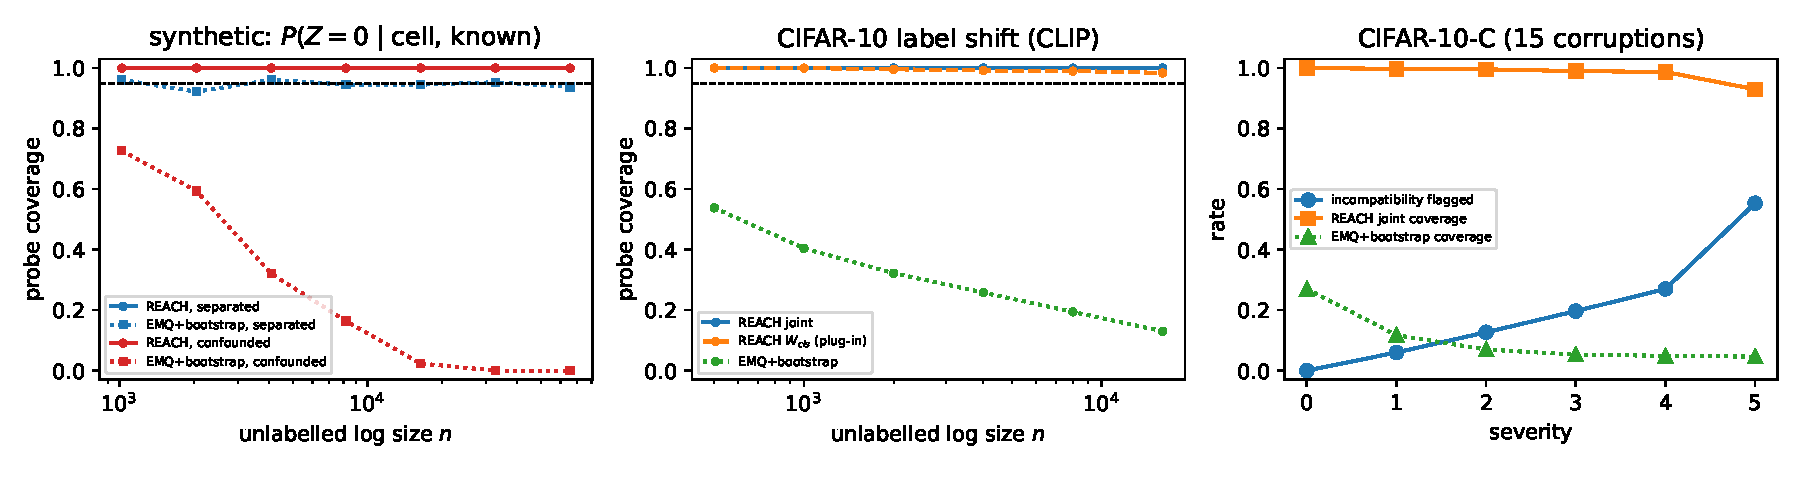
\includegraphics[width=\textwidth]{figures/fig3_coverage.pdf}
\caption{Per-probe inclusion of REACH and EMQ+bootstrap. Left: synthetic; both REACH curves lie on
$1.0$. Centre: CIFAR-10 label shift, four superclass sources. Right: CIFAR-10-C pooled over 15
corruptions, inclusion among runs where the ball is not empty, with the rate at which the
incompatibility test fires. Constraint-region and two-stage-bootstrap results are in the text.
Dashed: $0.95$.}
\label{fig:coverage}
\end{figure*}

\subsection{Does the width comparison choose the data that pays?}
\label{sec:exp-blindspot}

Without ground-truth widths this test is behavioural: take the acquisition REACH recommends per cell
and measure what it buys on held-out shifted data. Shift splits are clean CIFAR-10, CIFAR-10.1
\citep{recht2018cifar} and the 75 CIFAR-10-C splits, each cut into disjoint log, label and evaluation
pools. An episode draws Dirichlet(1) prevalences over the superclasses and starts from clean rows
($m=2000$) and $1000$ shifted log images. With budget $5000$ units, \emph{reweight} grows the log to
$6000$ and refits EMQ; \emph{add labels} buys $5000/c$ shifted labels and shrinks the rows towards them
($M_0=50$); \emph{do nothing} has payoff $0$. Payoff is the reduction of held-out negative
log-likelihood (nats) in a cell; regret is the best action's payoff minus the chosen one's. We compare
REACH (\cref{sec:setup}) with every constant policy, the incompatibility flag alone, and ensemble MI
mapped to actions by tercile with the map tuned on calibration-seed regret. Seeds 10--19 are
evaluated; intervals use a two-way cluster bootstrap over seeds and shift families. This is the second registered version of the test; the first had rule defects that review exposed
(\cref{app:deviations}).

\begin{table}[t]
\centering\small
\caption{Mean regret (nats per cell) by policy. Left: price 1:50 by shift family; right: all 77
splits at prices 1:50 and 1:250. Evaluation seeds; prior strength $M_0=50$.}
\label{tab:blindspot}
\setlength{\tabcolsep}{3pt}
\resizebox{\columnwidth}{!}{% generated from results/blindspot_v2/summary.json (evaluation seeds 10-19; prereg sha 2fdecf48)
\begin{tabular}{lrrrrr}
\toprule
 & \multicolumn{3}{c}{price 1:50, by family} & \multicolumn{2}{c}{all splits} \\
\cmidrule(lr){2-4}\cmidrule(lr){5-6}
policy & clean & C10.1 & C10-C & 1:50 & 1:250 \\
\midrule
REACH-v2 & 0.0029 & 0.0101 & 0.0864 & 0.0843 & 0.0411 \\
flag only & 0.0026 & 0.0096 & 0.0877 & 0.0856 & 0.0429 \\
always labels & 0.0086 & 0.0188 & 0.0100 & 0.0101 & 0.0084 \\
always reweight & 0.0019 & 0.0074 & 0.2382 & 0.2321 & 0.1189 \\
do nothing & 0.0018 & 0.0083 & 0.2401 & 0.2340 & 0.1208 \\
\bottomrule
\end{tabular}
}
\end{table}

\paragraph{Result.} The registered prediction fails: buying labels every time has lower regret than
REACH at every price ($0.010$ against $0.084$ at 1:50, difference CI $[0.038,0.134]$; $0.008$ against
$0.041$ at 1:250, $[0.014,0.063]$) and at every prior strength $M_0\in\{10,50,200\}$, and the regret-tuned
MI map is the same constant policy. The reason follows from the registered rule itself: under frozen
class-conditionals the predicted label gain can only widen the rows' radius when $n_k<m$ (true at every
price), so in a compatible frame REACH never predicts that labels help (largest predicted label gain $3\times10^{-8}$ at 1:50, $6\times10^{-8}$
over all settings). All of its label recommendations therefore come from the incompatibility test, which fires in only $33\%$ of
severity-5 episodes, while shifted labels pay $0.23$ nats under corruption. On clean CIFAR-10 and
CIFAR-10.1, where labels slightly hurt ($-0.007$ and $-0.011$ nats), REACH beats always-labels but not
doing nothing, always reweighting or the flag alone (\cref{tab:blindspot}); beyond the flag the width
comparison adds nothing (REACH minus flag-only within $[-0.005,0.0005]$ at 1:50). Under shift the widths
cannot tell whether the rows have moved.
% results/blindspot_v2/{summary.json,rows.csv.gz}; prereg real/blindspot_prereg_v2.py sha 2fdecf48

\subsection{When the class-conditionals hold: the exchange rate chooses the data}
\label{sec:exp-exchange}

Under frozen class-conditionals the question is which acquisition tightens a certified interval more at
a given price. Registered before its code and before a third encoder existed: $n_0\in\{500,2000,8000\}$,
$m_0\in\{125,500,2000\}$ ($\{32,128,512\}$ in a synthetic world with estimated rows), prices
$c\in\{10,50,250\}$, budget $5000$; the outcome is the realised reduction of the mean tight joint width.
REACH re-solves the tight interval at the post-acquisition radii; the data-free alternative compares the
radius reductions alone. Primary settings: the synthetic world and a frozen ResNet-50 \citep{he2016deep}
never inspected before the run; CLIP replicates; seeds 10--29 evaluated.

\begin{table}[t]
\centering\small
\caption{Exchange-rate test under pure label shift: which acquisition tightens the certified interval
more. Regret in width units, evaluation seeds; CI: seed bootstrap.}
\label{tab:exchange}
\setlength{\tabcolsep}{3pt}
\resizebox{\columnwidth}{!}{% generated from results/exchange_{synthetic,resnet50,clip}/summary.json and rows.csv.gz (prereg a70683e3)
\begin{tabular}{lccc}
\toprule
 & synthetic & ResNet-50 & CLIP \\
 & (blind) & (blind) & (seen) \\
\midrule
cells where labels are better & 14/27 & 4/27 & 4/27 \\
predicted sign correct & 1.00 & 1.00 & 1.00 \\
corr.\ predicted vs realised gain & 0.995 & 0.999 & 1.000 \\
\midrule
regret: REACH & 0.0019 & 0.0001 & 0.0001 \\
\quad radius bookkeeping & 0.0019 & 0.0000 & 0.0001 \\
\quad always log & 0.0540 & 0.0032 & 0.0035 \\
\quad always labels & 0.0487 & 0.0411 & 0.0426 \\
\quad ensemble MI (tuned) & 0.0224 & 0.0032 & 0.0035 \\
REACH $-$ best constant, 95\% CI & $[-0.0514,-0.0424]$ & $[-0.0036,-0.0026]$ & $[-0.0040,-0.0028]$ \\
\midrule
tight width (vs.\ region) & 0.83 (0.79) & 0.90 (0.89) & 0.89 (0.88) \\
tight $\le$ joint, share of probes & 1.00 & 1.00 & 1.00 \\
tight inclusion (min over bases) & 1.00 & 1.00 & 1.00 \\
\bottomrule
\end{tabular}
}
\end{table}

\paragraph{Result.} All registered claims hold (\cref{tab:exchange}), but what they establish is
narrower than the registration suggests. The better acquisition changes across base points and prices
in 14 of 27 synthetic cells and 4 of 27 real ones (labels win when the log is already large, references are
few and labels cheap), and REACH picks it, with regret below both constant policies and the tuned MI map
(CIs exclude zero in all three settings). Three qualifications. First, the decision value is the radius
exchange rate's: the data-free comparison of radii makes the same choice in $93$--$94\%$ of episodes with
regret equal to or lower than REACH's, and the choice is per deployment, not per input. Second, on real
features the stakes are small: ``always more log'' is right in 23 of 27 cells and trails by $0.003$ width
units on intervals about $0.9$ wide, and $29$--$32\%$ of episodes have mean width $\ge0.999$. Third, the
prediction re-solves the same program (partly a self-consistency check), and the tight interval, which
\cref{prop:bprime} does not cover, includes the target in every seed but stays wider than the constraint
region ($0.90$ against $0.89$ on ResNet-50).
% results/exchange_{synthetic,resnet50,clip}/summary.json; prereg real/exchange_prereg.py sha a70683e3

\subsection{Which source limits the certified interval?}
\label{sec:exp-attribution}

Attribution claims a per-input answer, so we score it against one. At each probe an \emph{oracle} removes
one source at a time from the tight joint interval (true marginal with tolerance $0$; true rows; true
$\delta$); the source whose removal narrows the interval most is the truth, scored where some removal narrows
it by at least $0.01$. Regret is the oracle's best narrowing minus that of the named source. The comparator
\emph{budget-majority} names the most frequent oracle source at the same setting and budget, learned with
hindsight on calibration seeds. Settings: the label-shift and held-out arms of \cref{sec:exp-real} with three
encoders (each CIFAR-10 class held out in turn; five CIFAR-100 superclasses), Gaussian features in
$\mathbb R^{64}$ through the same head, and classifier-like categorical worlds (\cref{app:details}).

\begin{table}[t]
\centering\small
\caption{Oracle regret (width units, evaluation seeds; on real data never run before the test was
registered) of naming the limiting source. Raw widths: argmax of $(\Wcls,\Wlab,\Wunk)$. Last data row: the realised
narrowing from acquiring $4\times$ more log or labels. CI: two-way bootstrap over seeds and settings.}
\label{tab:attribution}
\setlength{\tabcolsep}{3pt}
\resizebox{\columnwidth}{!}{\begin{tabular}{lcccc}
\toprule
 & raw widths & budget-majority & REACH-pin & pin $-$ majority [95\% CI] \\
\midrule
C10 held-out, 3 encoders & 0.284 & 0.045 & 0.0016 & $-0.043$ $[-0.047, -0.039]$ \\
C10 label shift, 3 encoders & 0.361 & 0.014 & 0.0012 & $-0.013$ $[-0.020, -0.007]$ \\
C100 held-out, CLIP & 0.400 & 0.009 & 0.0115 & $+0.002$ $[-0.003, +0.008]$ \\
C100 held-out, DINOv2 & 0.404 & 0.009 & 0.0028 & $-0.007$ $[-0.008, -0.005]$ \\
C100 label shift, CLIP & 0.307 & 0.001 & 0.0126 & $+0.011$ $[+0.005, +0.018]$ \\
C100 label shift, DINOv2 & 0.267 & 0.002 & 0.0041 & $+0.002$ $[-0.000, +0.005]$ \\
Gaussian features, held-out & 0.213 & 0.057 & 0.0125 & $-0.044$ $[-0.063, -0.026]$ \\
Classifier worlds (synthetic) & 0.266 & 0.022 & 0.0146 & $-0.007$ $[-0.010, -0.005]$ \\
C10 label shift, $4\times$ acquisition & 0.042 & 0.005 & 0.0005 & $-0.005$ $[-0.009, -0.002]$ \\
\midrule
C10 pooled (registered P1) & 0.298 & 0.039 & 0.0015 & $-0.038$ $[-0.043, -0.033]$ \\
\bottomrule
\end{tabular}
}
\end{table}

\paragraph{Result.} The published widths fail as an attribution: in a first registered test their argmax
was far worse than budget-majority ($0.28$ against $0.04$ on held-out CIFAR-10), because plug-in $\Wcls$ is
near $1$ at many probes limited by the rows. REACH-pin, registered afterwards and run on fresh seeds, passes
every registered claim (\cref{tab:attribution}): on CIFAR-10 its regret is $0.0015$ against $0.039$
($[-0.043,-0.033]$ for the difference) for every encoder and arm, accuracy $0.97$--$0.98$; it also wins with
Gaussian features, in classifier worlds, against a logistic map of the widths, and when the outcome is the
narrowing realised by buying $4\times$ more log or labels; the total interval includes its target throughout.
Where one source limits almost every input a constant does as well: on CIFAR-100 (rows limit
$90$--$99\%$) REACH-pin ties twice and loses once, and with $m=50$ labels per source it loses
(\cref{fig:a1,fig:a6}). The oracle shares REACH-pin's machinery, so this validates REACH-pin as an
estimator of the limiting source; the $4\times$ acquisition is the outcome outside that machinery.
% results/bridge/README.md (v1, prereg cd88f846); results/bridge2/README.md (prereg d8e97dab, amendment 9f4a189d);
% results/gauss/README.md (prereg fbbfe136)

\section{Limitations and outlook}
\label{sec:limitations}

REACH estimates no aleatoric uncertainty; its guarantees concern finitely many cells of a frozen
classifier, hold per budget, and rest on the declared mixture family, and on real features its intervals
are wide (\cref{sec:exp-real}). The raw widths are not on a common scale; the pinned rule fixes attribution
but beats a constant only where several sources compete. Choosing log or labels per deployment is a radius
exchange rate that data-free bookkeeping handles as well. Under shift the acquisition rule loses to a
constant, and a stronger incompatibility test is the main open problem: with Gaussian features shifted
inside the head's subspace (exploratory), inclusion is near $0.8$ at drift of one to two ball radii while
the test is silent (\cref{fig:a4}). Separation in feature space need not survive the frozen head
(\cref{fig:a3}). The unseen component is declared, and our data are one image family.


\subsection*{AI use statement}
In this work, we used generative AI tools to write and run experiment and analysis code, to help design
and write the pre-registration files, to draft Lean formalisations of the deterministic proof steps, to
search for and check related work, to run simulated peer reviews of drafts, and to draft and edit the text.
We did not use generative AI tools to generate the research question or the frozen abstract. We have
reviewed all AI-assisted work: every reported number is regenerated from the released scripts and result
files, the Lean statements are machine-checked with only Lean's standard axioms, every citation was checked
against the cited work, and the authors checked the proofs in the appendix. We take responsibility for the
final content of this work, including text, claims, or artifacts produced with the aid of generative AI.

\bibliographystyle{plainnat}
\bibliography{refs}

\section*{Checklist}

\begin{enumerate}
  \item For all models and algorithms presented, check if you include:
  \begin{enumerate}
    \item A clear description of the mathematical setting, assumptions, algorithm, and/or model. Yes
    (\cref{sec:setup,sec:theory}).
    \item An analysis of the properties and complexity (time, space, sample size) of any algorithm. Yes:
    each interval endpoint is one cone or linear program in $K+1$ variables with $d$ cells, and the radii
    give the sample-size dependence (\cref{sec:setup,lem:ball}, \cref{app:details}).
    \item (Optional) Anonymized source code, with specification of all dependencies, including external
    libraries. Yes (supplementary material).
  \end{enumerate}
  \item For any theoretical claim, check if you include:
  \begin{enumerate}
    \item Statements of the full set of assumptions of all theoretical results. Yes (\cref{sec:theory}).
    \item Complete proofs of all theoretical results. Yes (\cref{app:proofs}); deterministic and
    measure-theoretic cores are also machine-checked in Lean (\cref{app:lean}).
    \item Clear explanations of any assumptions. Yes (\cref{sec:setup,sec:theory}).
  \end{enumerate}
  \item For all figures and tables that present empirical results, check if you include:
  \begin{enumerate}
    \item The code, data, and instructions needed to reproduce the main experimental results. Yes
    (supplementary code, pre-registration files and commands; public datasets).
    \item All the training details (e.g., data splits, hyperparameters, how they were chosen). Yes
    (\cref{sec:experiments}, \cref{app:details}); nothing is trained beyond a PCA and LDA head on a fixed
    development split, and every design choice made after seeing results is listed in
    \cref{app:deviations}.
    \item A clear definition of the specific measure or statistics and error bars. Yes: bootstrap
    intervals over seeds, or over seeds and shift families (\cref{sec:experiments}).
    \item A description of the computing infrastructure used. Yes (\cref{app:details}).
  \end{enumerate}
  \item If you are using existing assets (e.g., code, data, models) or curating/releasing new assets,
  check if you include:
  \begin{enumerate}
    \item Citations of the creator if your work uses existing assets. Yes (CIFAR-10, CIFAR-10-C, CIFAR-10.1,
    CIFAR-100, CLIP, DINOv2, ResNet-50).
    \item The license information of the assets, if applicable. Yes, in the supplementary README.
    \item New assets either in the supplemental material or as a URL, if applicable. Yes (code,
    pre-registration files, Lean project).
    \item Information about consent from data providers/curators. Not Applicable.
    \item Discussion of sensible content if applicable. Not Applicable.
  \end{enumerate}
  \item If you used crowdsourcing or conducted research with human subjects, check if you include:
  \begin{enumerate}
    \item The full text of instructions given to participants and screenshots. Not Applicable.
    \item Descriptions of potential participant risks, with links to IRB approvals if applicable. Not
    Applicable.
    \item The estimated hourly wage paid to participants and the total amount spent on participant
    compensation. Not Applicable.
  \end{enumerate}
\end{enumerate}


\clearpage
\appendix
\onecolumn

\section{Proofs}
\label{app:proofs}

\paragraph{Distinguishability facts.} (a) $\sigma(A)>0$ iff no nonzero $v\in T$ has $v^{\top}A=0$, i.e.\
iff the rows are affinely independent. (b) $\sigma(A)\le s$: let $c^{*}\in\Delta_K$ attain
$s=\lVert q-\sum_kc^{*}_kA_k\rVert$ and $v=(e_{K+1}-c^{*})/\lVert e_{K+1}-c^{*}\rVert$, a unit tangent
vector; then $\lVert v^{\top}A\rVert=s/\sqrt{1+\lVert c^{*}\rVert^2}\le s$. (c) For any unit $v\in T$,
$\lVert v^{\top}\hat A\rVert\ge\lVert v^{\top}A\rVert-\sum_k|v_k|\lVert\hat A_k-A_k\rVert\ge\sigma(A)-\sqrt{K+1}\,r$.

\paragraph{Lemma~\ref{lem:ball}.} Write $\hat p_n=\frac1n\sum_{i}e_{X_i}$. By Jensen,
$\mathbb E\lVert\hat p_n-p^{*}\rVert_2\le(\mathbb E\lVert\hat p_n-p^{*}\rVert_2^2)^{1/2}
=((1-\lVert p^{*}\rVert_2^2)/n)^{1/2}\le n^{-1/2}$. Replacing one draw moves $\hat p_n$ by at most
$\sqrt2/n$ in $\ell_2$, so by McDiarmid's inequality
$\Pr(\lVert\hat p_n-p^{*}\rVert_2\ge n^{-1/2}+t)\le\exp(-nt^2)$; the choice
$t=\sqrt{\log(1/\alpha)/n}$ suffices, and the stated $\varepsilon_n$ with $\sqrt{2\log(1/\alpha)}$
is larger by a factor $\sqrt2$ on the deviation term, hence also valid.
On this event and (L3), for $w^{*}\in\Delta_{K+1}$,
$\lVert w^{*\top}\hat A-\hat p_n\rVert\le\lVert\sum_kw^{*}_k(\hat A_k-A_k)\rVert+\lVert p^{*}-\hat p_n\rVert
\le\sum_kw^{*}_k r+\varepsilon_n=\varepsilon_n+r$ (Lean: \texttt{ball\_contains\_truth}). Every
interval over $\mathcal W_n$ then contains the value at $w^{*}$; intervals that also range over
label-channel or component intervals contain the target on the intersection of their events, whose
failure probability is bounded by the union bound used to split $\alpha$.

\paragraph{Proposition~\ref{prop:bprime}.} For $w,w'\in\mathcal W_n$, $v=w-w'\in T$ and
$\lVert v^{\top}\hat A\rVert\le\lVert w^{\top}\hat A-\hat p_n\rVert+\lVert w'^{\top}\hat A-\hat p_n\rVert
\le2(\varepsilon_n+r)$, so $\sigma\lVert v\rVert_2\le2(\varepsilon_n+r)$ (Lean: \texttt{diam\_bound}).
At a probe, $f(w)=u(w)/v(w)$ with $u=w_ka_k$, $v=\sum_{j\le K}w_ja_j$, $a_j=\hat A_j(x)\in[0,a_{\max}]$.
For $0\le u'\le v'$ and $v,v'>0$, $|u/v-u'/v'|\le(|u-u'|+|v-v'|)/v$ (Lean: \texttt{ratio\_lipschitz}),
and $|u-u'|,|v-v'|\le a_{\max}\lVert w-w'\rVert_1$, so
$|f(w)-f(w')|\le2a_{\max}\lVert w-w'\rVert_1/v(w)$ (Lean: \texttt{posterior\_lipschitz}). With
$\lVert\cdot\rVert_1\le\sqrt{K}\lVert\cdot\rVert_2$ on the $K$ known coordinates, the only ones that
enter $f$, and $v(w)\ge\min_{\mathcal W_n}v$, the width is at most
$L(x)\,2(\varepsilon_n+r)/\sigma$. The rates follow from $\varepsilon_n=O(n^{-1/2})$ and
$r=O(m^{-1/2})$.

\paragraph{Proposition~\ref{prop:b}.} Under (B1)--(B2) the log's law is that of $n$ i.i.d.\ draws from
$w^{*\top}A$, in which $\theta$ does not appear, so it is the same law $P$ under $\theta$ and $\theta'$.
Let $C(\cdot)$ be a procedure that uses only the log with $P(\vartheta\notin C)\le\alpha$ for
$\vartheta\in\{\theta,\theta'\}$. Then $P(\theta\in C,\theta'\in C)\ge1-P(\theta\notin C)-P(\theta'\notin C)
\ge1-2\alpha$, by subadditivity of outer measure, so no measurability of $C$ is needed. On that event
the interval has width at least $|\theta_k-\theta'_k|$, and for the label posterior at fixed shares
$\pi_k(x)$ at least $|\sum_k\pi_k(x)(\theta_k-\theta'_k)|$ (Lean: \texttt{two\_point}, \texttt{width\_ge};
the Lean statement assumes coverage at every parameter value, which is stronger than at two). For the rate, each source's
noisy label mean has Hoeffding half-width $\sqrt{\log(2K/\alpha)/(2m)}$ and debiasing a known
symmetric flip divides it by $1-2\eta$.

\paragraph{Proposition~\ref{prop:c}.} (i) As for \cref{prop:bprime} with $u=w_{K+1}q(x)$ and
$v=w^{\top}\hat A(x)$, using (C1) for the diameter and (C2) for the denominator. (ii) Let
$q=\sum_kc_kA_k$ with $c\in\Delta_K$, extended by $c_{K+1}=0$. For $w_t=w^{*}+t(e_{K+1}-c)$,
$w_t^{\top}A=w^{*\top}A$ for all $t$ and $(w_t)_{K+1}=w^{*}_{K+1}+t$ (Lean:
\texttt{novel\_not\_identified}); $w_t\in\Delta_{K+1}$ for $0\le t\le\min_{k:c_k>0}w^{*}_k/c_k$,
which is positive when $w^{*}$ has slack (Lean: \texttt{novel\_segment\_in\_simplex}). On the event of
\cref{lem:ball}, $\lVert w_t^{\top}\hat A-\hat p_n\rVert\le\lVert w_t^{\top}(\hat A-A)\rVert+\lVert p^{*}-\hat p_n\rVert
\le r+\varepsilon_n$, so every $w_t$ lies in $\mathcal W_n$. For $q(x)>0$ the coverage posterior
$w_{K+1}q(x)/w^{\top}A(x)$ is strictly increasing along the segment (the denominator is constant), so
$\Wunk(x)$ is at least its increase over the segment, a positive constant independent of $n$. This
uses the true rows in the posterior: it holds for $\Wunk$ when rows are known ($r=0$, the synthetic
study) and for the joint coverage interval, which ranges over the true entries, when they are
estimated. We do not claim convergence of $\Wunk(x)$ to a limit. (iii) is the stated policy.

\paragraph{Noisy labels on real data.} Each reference label is flipped with known probability $\eta$
to a uniformly chosen other source. With $T_l=\frac1m\sum_i\mathbf 1\{\tilde y_i=l\}e_{\mathrm{cell}(i)}$,
$\mathbb ET=MA$ with $M=(1-\eta)I+\frac{\eta}{K-1}(\mathbf 1\mathbf 1^{\top}-I)$, invertible for
$\eta<(K-1)/K$, and $\hat A=\Pi_\Delta(M^{-1}T)$ row-wise, where Euclidean projection onto the
simplex cannot increase the distance to a simplex row. The error of $T_l$ splits into cell sampling
given which images landed under label $l$ (McDiarmid over the $n_l$ landed images) and the deviation
of the landing counts $c_{jl}\sim\mathrm{Bin}(m,M_{jl})$, bounded by Bernstein's inequality and
vanishing as $\sqrt\eta$. $M^{-1}$ amplifies a row error by at most $\lVert M^{-1}\rVert_\infty$.

\section{Machine-checked statements}
\label{app:lean}

The supplementary Lean~4 project (Mathlib, pinned) checks the following; \texttt{\#print axioms}
reports only \texttt{propext}, \texttt{Classical.choice} and \texttt{Quot.sound} for each, and the file
contains no \texttt{sorry}.

\begin{center}\small
\resizebox{\textwidth}{!}{\begin{tabular}{lll}
\toprule
Lean theorem & Statement & Used in \\
\midrule
\texttt{ball\_contains\_truth} & concentration event $\Rightarrow w^{*}$ satisfies the ball constraint & Lemma~\ref{lem:ball} \\
\texttt{diam\_bound}, \texttt{simplex\_sub\_sum\_zero} & $\sigma\lVert w-w'\rVert\le2\rho$ on the tangent space & Prop.~\ref{prop:bprime} \\
\texttt{ratio\_lipschitz}, \texttt{posterior\_lipschitz} & posterior moves by $\le2a_{\max}\lVert w-w'\rVert_1/v$ & Prop.~\ref{prop:bprime}, \ref{prop:c}(i) \\
\texttt{two\_point}, \texttt{width\_ge} & same log law $\Rightarrow$ width $\ge|\theta-\theta'|$ & Prop.~\ref{prop:b} \\
\texttt{novel\_not\_identified}, \texttt{novel\_segment\_in\_simplex} & $q$ in the hull $\Rightarrow$ non-identified segment & Prop.~\ref{prop:c}(ii) \\
\bottomrule
\end{tabular}}
\end{center}
Not formalised: the concentration inequality (Mathlib provides no McDiarmid inequality), the
$\ell_1$--$\ell_2$ conversion, and the label-channel rates.

\section{Implementation details}
\label{app:details}

\paragraph{Cells and head.} Features are L2-normalised CLIP ViT-B/32 or DINOv2 ViT-S/14 image
embeddings of bicubic-resized $224\times224$ images, extracted once and frozen. PCA to 32 dimensions
and a pooled-covariance Gaussian discriminant with equal class priors are fitted on a fixed
$10{,}000$-image development split; the outlier cell collects inputs whose smallest Mahalanobis
distance exceeds the development 99th percentile.

\paragraph{Radii and budget.} $\alpha=0.05$ is split equally between the log, the references and the
label channel; the reference share is split over the $K+1$ rows and the label-channel share over the
$K\times d$ entries, each with a Hoeffding interval. The ball is solved without relaxation (second-order cone,
Clarabel); the coordinate box outer approximation gives the same synthetic decisions but is about
$30\%$ wider there and close to vacuous with ten sources.

\paragraph{Baselines on real data.} The constraint region follows the construction of
\citet{li2026matrix}: weights in the simplex satisfying, for every cell, $\sum_j\underline A_j(x)w_j\le\hat
p_n(x)+t$ and $\sum_j\overline A_j(x)w_j\ge\hat p_n(x)-t$, with $t$ a Hoeffding half-width for the log
frequencies (union over cells, budget $\alpha/3$) and $[\underline A,\overline A]$ the same per-entry intervals
as REACH's joint interval. Posterior extrema over it are linear-fractional programs solved as LPs. It
is our reimplementation from the paper's description, not the authors' code. The two-stage bootstrap
resamples each reference row ($m$ multinomial draws) and the log, refits EMQ, and takes percentile
intervals (200 replicates).

\paragraph{Tight joint interval.} With $u=tw$ and slack $s\ge0$, each endpoint solves
$\min/\max\ \text{num}^{\top}u$ subject to $s_c\ge\sum_ju_j\underline A_j(c)-t\hat p_n(c)$,
$s_c\ge t\hat p_n(c)-\sum_ju_j\overline A_j(c)$, $\lVert s\rVert_2\le t\varepsilon_n$, $\mathbf 1^{\top}u=t$,
$\text{den}^{\top}u=1$ (Clarabel). Validity: on the event of \cref{lem:ball} and the entry events the
true marginal $\sum_jw^{*}_jA_j$ lies in the box, so its distance from $\hat p_n$ is at most
$\varepsilon_n$. The constraint region of \cref{sec:exp-real} uses per-cell intervals on the log
(share $\alpha/3$) and the entry intervals (share $\alpha/3$); the tight interval spends the same $2\alpha/3$,
while the joint interval also spends a third share on the row radius $r$. The tight interval is not
provably nested in the joint interval (the entry box can have a larger Euclidean diameter than $r$); that it
is never wider in our runs is an empirical finding.

\paragraph{Acquisition test (version 2).} Pools are 50/20/30\% log/label/evaluation, fixed per split.
Component entries are floored at $10^{-4}$ before computing posteriors so the log-likelihood is
finite. Shifted labels update rows as $(M_0\hat A_k+\text{counts}_k)/(M_0+n_k)$. Ensemble MI uses 20
members that resample the log and the references; its tercile-to-action map is chosen among all 27 maps
over three actions by calibration-seed regret. Evaluation risk is importance-weighted to the episode's
prevalences. Because the prevalences and the clean rows depend only on the seed, episodes from
different splits are not independent; intervals use a two-way cluster bootstrap over seeds and shift
families.

\paragraph{Oracle removal and pinning (\cref{sec:exp-attribution}).} The total interval is the tight
joint interval of $P(\text{source}=\hat y(x)\mid x)$ over all sources, known and unseen. Oracle removals:
log, histogram set to $w^{*\top}A$ and tolerance $0$; rows, every entry interval collapsed to the true row
of the deployment pool (the unseen row included); unseen, the constraint $w_{K+1}=\delta$. Pinned removals
use the current estimates instead: $w_0=\arg\min_w\operatorname{dist}(\hat p_n,\text{box}(w))$ and the
nearest box point $x_0$ (log); $\hat A$ with tolerance $\max(\varepsilon_n,\text{best-fit residual})$ so the
set is non-empty (rows); $w_{K+1}=w_{0,K+1}$ (unseen). A removal that empties the set is never named.
Budget-majority and the logistic map of the widths are fitted on calibration seeds $0$--$9$; real evaluation
seeds are $30$--$59$, run for the first time in this test. The finite-acquisition outcome compares the
realised narrowing from $n\to4n$ and $m\to4m$ at $m\in\{125,500\}$ on the CIFAR-10 label-shift settings.

\paragraph{Classifier worlds.} $K$ known sources, \emph{per} cells per source and one outlier cell
($d=K\cdot\text{per}+1$); row $k$ puts mass $a$ (accuracy) on its own cells, split by a Dirichlet(1) draw,
and $1-a$ on Dirichlet(1) noise over all cells, with the outlier entry down-weighted fivefold. The unseen
row is $\lambda(\tfrac12e_{\text{outlier}}+\tfrac12\text{Dir}(1))+(1-\lambda)$ times a random mixture of
known rows. $(K,\text{per})\in\{(3,1),(3,3),(6,1),(6,2),(10,1)\}$, $a\in\{0.6,0.8,0.95\}$,
$\lambda\in\{0,0.3,1\}$, four draws each; $n\in\{500,5000,50000\}$, $m\in\{50,500,5000,50000\}$; the unseen
row is estimated from 2000 draws. The dose-response study uses the same recipe with $K=4$, per $=1$.

\paragraph{Gaussian-feature world.} Features $x\sim\mathcal N(\mu_c,I_{64})$, $5000$ training and $2000$
test points per class, four known classes with $\mu_k=\Delta u_k$ for random unit $u_k$, and an unseen
class at $\lambda\Delta u_{\text{new}}+(1-\lambda)(\mu_0+\mu_1)/2$, $\Delta\in\{1.5,2.5,4\}$,
$\lambda\in\{0,0.5,1\}$, three draws. They pass through exactly the head and audit code used for CIFAR.
Covariate shift adds $\tau v$ to the test features: in the registered design $v$ is a random unit vector,
in the exploratory run it is $u_0$.

\paragraph{Compute.} The synthetic study runs on a laptop CPU in minutes. Feature extraction ran on one
A10G GPU; the real audits and the blind-spot test ran on 32-core CPU containers, each in under an
hour.

\section{Additional results}
\label{app:extra}

\begin{figure}[h]
\centering
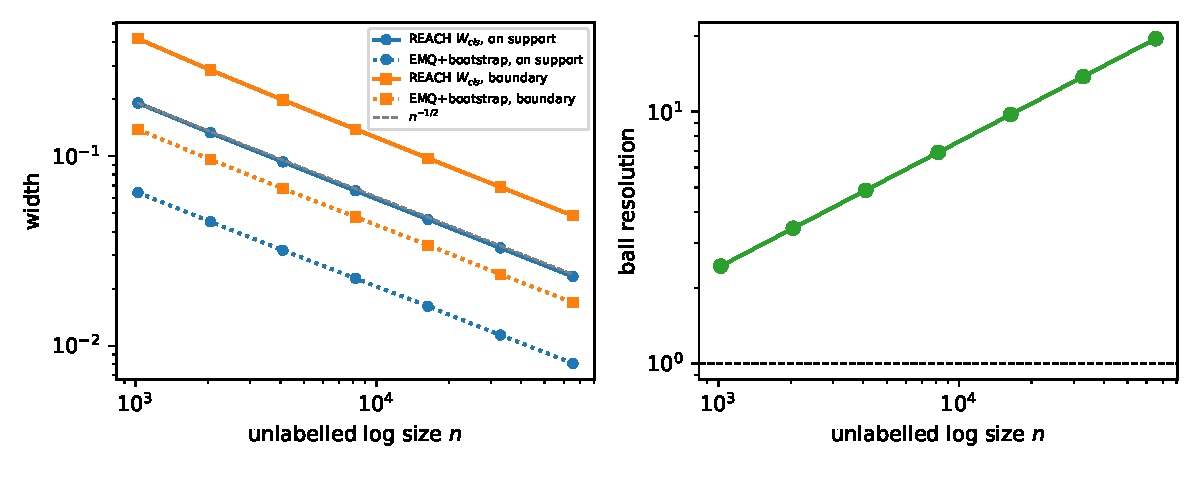
\includegraphics[width=.75\textwidth]{figures/fig2_wcls_vs_n.pdf}
\caption{Synthetic, world \emph{separated}. Left: $\Wcls$ (solid) and EMQ+bootstrap width (dotted)
against $n$; dashed slope $-1/2$. Right: ball resolution, which must exceed $1$ at the smallest $n$.}
\end{figure}

\paragraph{Second backbone.} With DINOv2 ViT-S/14 \citep{oquab2024dinov2} the head is $95.2\%$
accurate and the resolution gate reads $1.22$ (super4) and $1.75$ (ten sources). 13 of 13 registered
cells agree (12 of 13 with ten sources, the same saturated noise cell). The joint interval and the
constraint region cover in every seed in every label-shift and unseen-class arm; at $n=16{,}000$ their
widths are $0.69$ and $0.63$ (super4; $0.86$ and $0.72$ with ten sources), and the two-stage bootstrap
covers $0.74$ ($0.68$). Plug-in $\Wunk$ covers $0.89$ and $0.88$ when unseen classes are present; the
joint coverage interval covers in every seed. The corruption arm was not repeated for DINOv2.

\paragraph{Label noise (CLIP, super4).} Over $\eta\in\{0.025,\dots,0.3\}$ the joint interval and the
constraint region cover in every seed and both widen to $1.00$ (joint $0.92\to1.00$); the two-stage
bootstrap covers between $0.42$ and $0.73$.

\paragraph{Corruption--severity cells with joint coverage below $0.95$} (CLIP; coverage among answered
runs, and the rate at which the incompatibility test fires). \emph{four superclass sources}: elastic transform 5 (0.74, flag 0.35); frost 5 (0.90, flag 0.40); glass blur 1 (0.70, flag 0.90); glass blur 2 (0.70, flag 0.90); glass blur 3 (0.70, flag 0.85); jpeg compression 4 (0.95, flag 0.05); jpeg compression 5 (0.87, flag 0.35); motion blur 4 (0.94, flag 0.00); motion blur 5 (0.85, flag 0.45); pixelate 5 (0.80, flag 0.75).

\emph{ten class sources}: contrast 5 (0.80, flag 0.95); elastic transform 5 (0.92, flag 0.00); fog 5 (0.90, flag 0.00); frost 5 (0.94, flag 0.00); gaussian noise 2 (0.90, flag 0.00); gaussian noise 3 (0.81, flag 0.00); gaussian noise 4 (0.81, flag 0.00); gaussian noise 5 (0.80, flag 0.00); glass blur 1 (0.90, flag 0.00); glass blur 2 (0.90, flag 0.00); glass blur 3 (0.90, flag 0.00); glass blur 4 (0.86, flag 0.00); glass blur 5 (0.85, flag 0.00); impulse noise 4 (0.84, flag 0.00); impulse noise 5 (0.80, flag 0.00); jpeg compression 5 (0.94, flag 0.00); motion blur 5 (0.92, flag 0.00); pixelate 5 (0.93, flag 0.00); shot noise 3 (0.85, flag 0.00); shot noise 4 (0.83, flag 0.00); shot noise 5 (0.81, flag 0.00).

\paragraph{Where \cref{prop:c} stops: CIFAR-100.} Known sources are four trees (maple, oak, palm, pine)
and five vehicles, grouped into two sources; the novel source ($\delta=0.1$) is willow, a sibling of
the known trees, or whale. We registered that willow should show a smaller separation $s$, a flatter
$\Wunk$ slope and a wider final $\Wunk$ than whale. With 400 reference images per class the novel
row's radius alone is about $0.21$ and the resolution gate passes only for $n\ge8000$, so this arm is
descriptive. With CLIP all three predictions hold ($s=0.30$ vs $0.46$; slope $-0.02$, inside the
placebo band, vs $-0.09$; final width $0.57$ vs $0.51$). With DINOv2 only the slope prediction holds
($-0.03$ vs $-0.06$): in that encoder's cells willow is further from the known hull than whale
($s=0.35$ vs $0.32$). The joint novelty interval covers in all four runs. Whether a sibling class is
inside the support is a property of the representation, not of the label hierarchy.

\section{All pre-registered outcomes}
\label{app:outcomes}

\Cref{tab:outcomes-early,tab:outcomes-late} list every registered prediction with its outcome. Of the 24
directional claims registered for the attribution, Gaussian-feature and dose-response studies, 17 hold and
7 fail; the failures and their likely causes are plotted in \cref{fig:a1,fig:a2,fig:a3,fig:a4,fig:a5,fig:a6}.
Numbers are evaluation-seed means; brackets are 95\% bootstrap intervals.

\begin{table}[!htbp]
\centering\footnotesize
\caption{Registered outcomes of the tests in \cref{sec:exp-synthetic,sec:exp-real,sec:exp-blindspot,sec:exp-exchange}.}
\label{tab:outcomes-early}
\begin{tabular}{p{3.4cm}p{8.2cm}p{1.6cm}}
\toprule
test & outcome & verdict \\
\midrule
Synthetic response matrix & 23 of 25 cells agree; 12 baseline cells agree; of 7 non-trivial REACH cells 5 agree & 2 FAIL \\
\quad $\Wunk$, \emph{confounded} & registered ``no response''; slopes $-0.09$ (on support), $-0.04$ (boundary): attenuated, bounded below & FAIL \\
CIFAR-10 audit (CLIP, DINOv2) & 13/13 cells (super4); 12/13 (ten sources: saturated noise cell) & 1 FAIL each \\
CIFAR-100 limit arm & CLIP 3/3 predictions; DINOv2 1/3 (sibling class further from hull) & 2 FAIL \\
Acquisition under shift (v2) & REACH regret $0.084$ vs always-labels $0.010$ at 1:50 & FAIL \\
Exchange rate E1--E4 & all hold on synthetic and blind ResNet-50 & PASS \\
\bottomrule
\end{tabular}
\end{table}

\begin{table}[!htbp]
\centering\footnotesize
\caption{Registered outcomes of the attribution (v1, v2), Gaussian-feature (G) and dose-response (D)
studies. Pre-registrations: \texttt{real/bridge\_prereg.py}, \texttt{real/bridge2\_prereg.py} with
\texttt{real/bridge2\_amendment.py}, \texttt{real/gauss\_dose\_prereg.py}.}
\label{tab:outcomes-late}
\begin{tabular}{p{4.6cm}p{7.6cm}p{1.2cm}}
\toprule
claim & outcome & verdict \\
\midrule
v1 A1/A2: raw-width argmax beats budget-majority & regret $0.280$ vs $0.043$ (held-out), $0.356$ vs $0.015$ (label shift) & FAIL \\
v1 D1: $\Wcls$ falls with $\sigma(\hat A)$ & coefficient $+1.10$ $[1.02,1.23]$; confounded by $K$ (\cref{fig:a2}); B$'$ bound holds but never $<1$ & FAIL \\
v1 D2: $\Wunk$ falls with $s$ (40 candidates) & Spearman $-0.03$ $[-0.14,0.11]$; pooled across $K$ (\cref{fig:a3}) & FAIL \\
v1 D3: $\Wlab$ includes, tracks row error & inclusion $1.000$; positive in 21/24 & PASS \\
v1 D4: drift ratio $\rho$ vs inclusion, flag & Spearman $-0.72$, $+0.65$ (\cref{fig:a4}) & PASS \\
v2 P1: REACH-pin beats budget-majority (C10) & $-0.038$ $[-0.043,-0.033]$ & PASS \\
v2 P2/P3: same, classifier worlds; accuracy $\ge0.7$ & $-0.0075$ $[-0.010,-0.005]$; $0.91$ & PASS \\
v2 P4: same, $4\times$ acquisition & $-0.005$ $[-0.009,-0.002]$ & PASS \\
v2 P6: inclusion $\ge0.95$ & $1.000$ in every arm & PASS \\
G1: REACH-pin beats budget-majority & $-0.044$ $[-0.063,-0.026]$ & PASS \\
G2: inclusion & $1.000$ & PASS \\
G3: $\rho$ vs inclusion, flag & registered shifts too weak ($\rho\le0.35$), flag never fires (\cref{fig:a4}) & FAIL \\
G4a: $\Wcls$ falls with $\Delta$ & Spearman $-0.89$ $[-0.94,-0.77]$ & PASS \\
G4b: $\Wunk$ falls with $s$ & Spearman $+0.41$ $[0.28,0.57]$; $s\le0.2$ in every world (\cref{fig:a3}) & FAIL \\
Dcls-1: $n$-rate of $\Wcls$ in $[-0.75,-0.25]$ & $-0.40$ $[-0.41,-0.38]$ & PASS \\
Dcls-2: $\Wcls$ falls with $\sigma$, $K$ fixed & slope $-0.65$ $[-0.88,-0.52]$ (\cref{fig:a2}) & PASS \\
Dcls-3: lower probe mass, wider $\Wcls$ & 93\% of worlds & PASS \\
Dlab-1: $\Wlab$ monotone in $\eta$ (Spearman $=1$ in $\ge80\%$) & $67\%$; non-decreasing in 36/36, failures are ties at $\Wlab=1$ (\cref{fig:a5}) & FAIL \\
Dlab-2: label-interval inclusion & $1.000$ at every $\eta$ & PASS \\
Dlab-3: $\Wlab$ tracks realised error & Spearman $0.30$, positive in 36/36 & PASS \\
Dunk-1: $\Wunk$ falls with $s$, $K$ fixed & Spearman $-0.97$ $[-0.97,-0.94]$ (\cref{fig:a3}) & PASS \\
Dunk-2: no contraction at $s=0$; contraction for large $s$ & slopes $-0.095$ (bound $-0.1$, narrowly) and $-0.53$ & PASS \\
\bottomrule
\end{tabular}
\end{table}

\begin{figure}[!htbp]
\centering
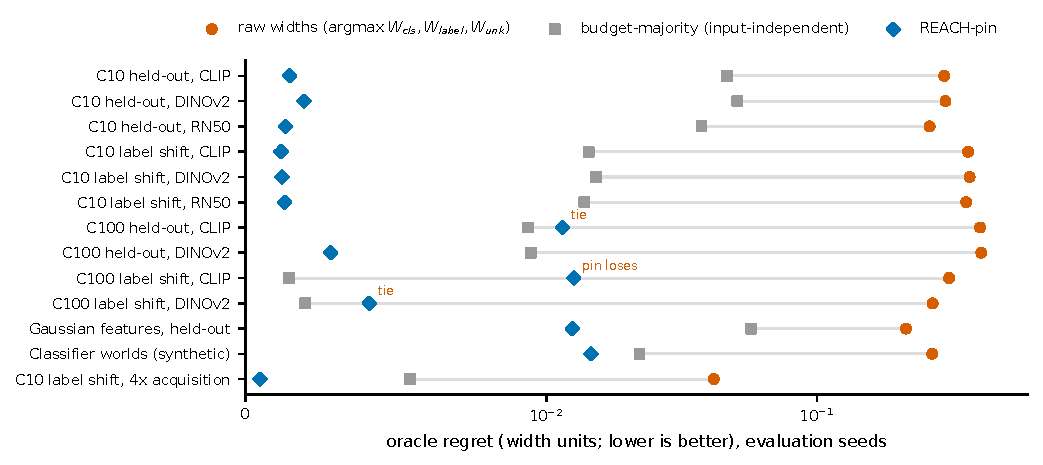
\includegraphics[width=.9\textwidth]{figures/figA1_attribution.pdf}
\caption{Oracle regret of naming the limiting source, per setting (log scale near $0$). REACH-pin beats
budget-majority on every CIFAR-10 setting, the Gaussian world, the classifier worlds and the $4\times$
acquisition outcome; on CIFAR-100, where the rows limit 90--99\% of inputs, it ties twice and loses once
(CI excluding $0$). The raw-width argmax is worst everywhere.}
\label{fig:a1}
\end{figure}

\begin{figure}[!htbp]
\centering
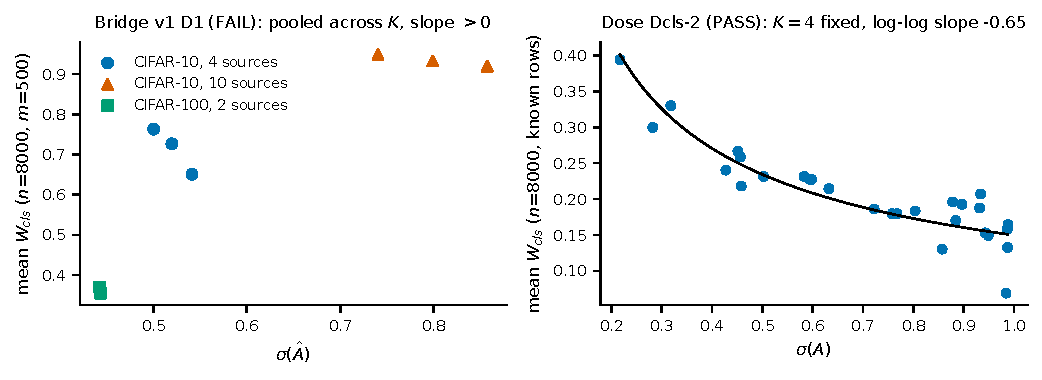
\includegraphics[width=.9\textwidth]{figures/figA2_sigma.pdf}
\caption{Prevalence width and distinguishability. Left (registered v1 D1, failed): pooling real settings
with different numbers of sources gives a positive slope, because ten-source settings have larger
$\sigma$ but smaller per-class mass. Right (Dcls-2, passed): with $K=4$ fixed, $\Wcls$ falls with $\sigma$.}
\label{fig:a2}
\end{figure}

\begin{figure}[!htbp]
\centering
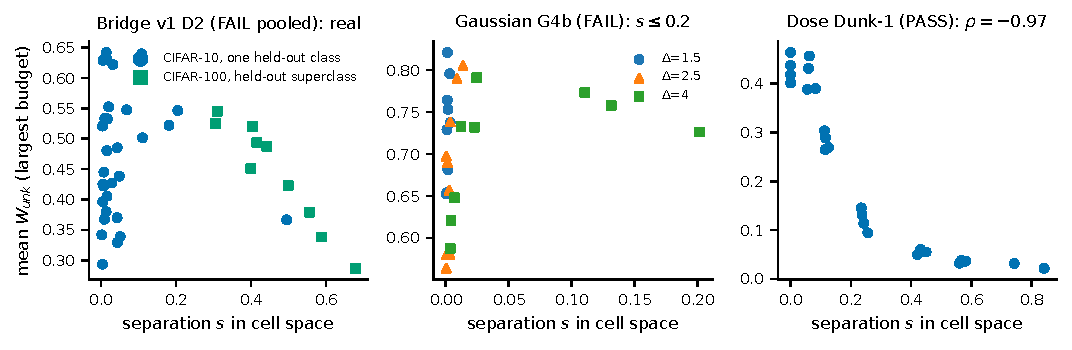
\includegraphics[width=\textwidth]{figures/figA3_separation.pdf}
\caption{Coverage width and separation in cell space. Left (v1 D2, failed pooled): real held-out classes;
within CIFAR-100 ($K=2$) the width falls with $s$. Centre (G4b, failed): Gaussian features; the head's PCA
projects the novel direction away, so $s\le0.2$ and the width follows how diffusely the novel class spreads.
Right (Dunk-1, passed): categorical worlds with $K=4$ fixed.}
\label{fig:a3}
\end{figure}

\begin{figure}[!htbp]
\centering
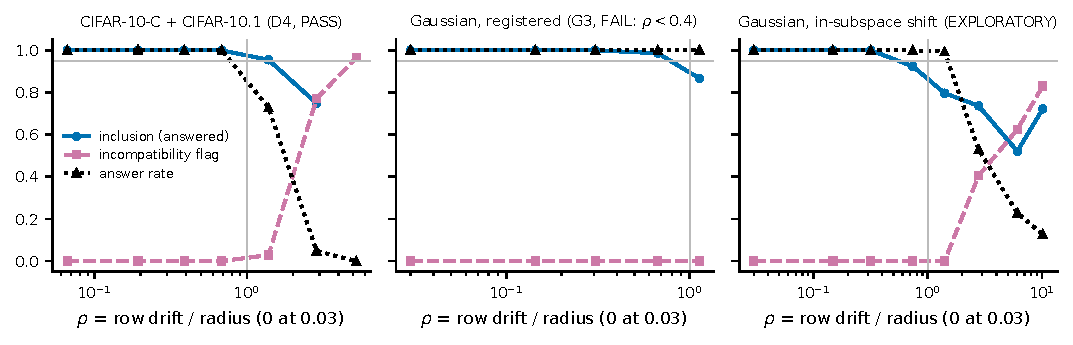
\includegraphics[width=\textwidth]{figures/figA4_shift.pdf}
\caption{Inclusion among answered runs, incompatibility-flag rate and answer rate against $\rho$, the row
drift in units of the ball radius (binned). Left: CIFAR-10-C and CIFAR-10.1 (registered, passed). Centre:
registered Gaussian shifts, too weak to reach $\rho=1$ (failed). Right (exploratory, not registered):
shift inside the head's subspace; inclusion falls to $0.92$ at $\rho\in(0.5,1]$ and $0.80$ at $\rho\in(1,2]$
before the flag fires.}
\label{fig:a4}
\end{figure}

\begin{figure}[!htbp]
\centering
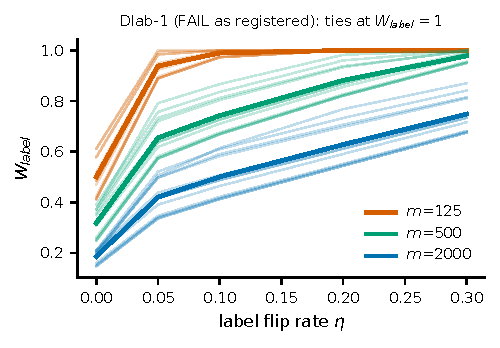
\includegraphics[width=.5\textwidth]{figures/figA5_label_noise.pdf}
\caption{Label width against label noise (Dlab-1, failed as operationalised). Thin lines: worlds; thick:
means. The width never decreases in $\eta$; at $m=125$ it saturates at $1$, and the resulting ties fail the
registered ``Spearman $=1$'' criterion.}
\label{fig:a5}
\end{figure}

\begin{figure}[!htbp]
\centering
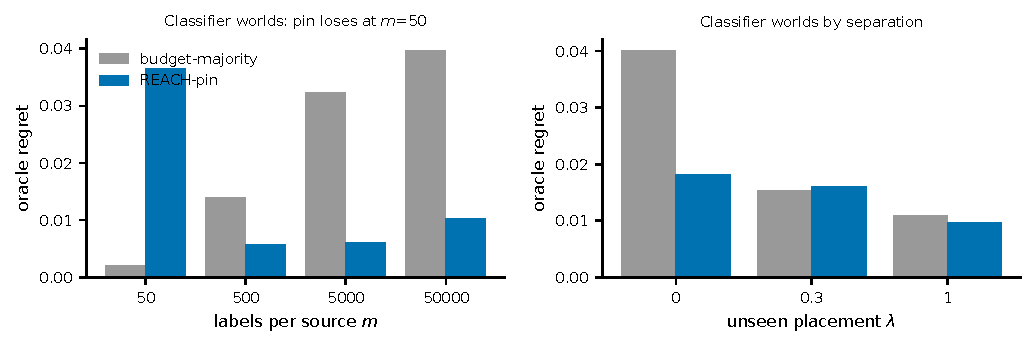
\includegraphics[width=.9\textwidth]{figures/figA6_pin_limits.pdf}
\caption{Where REACH-pin does not help (classifier worlds). Left: with $m=50$ labels per source the rows
limit almost every input and the pinned rows are poor, so pinning loses to budget-majority. Right: by
placement of the unseen source.}
\label{fig:a6}
\end{figure}

\clearpage
\section{Pre-registration and deviations}
\label{app:deviations}

Expected outcomes were committed in code before each test ran, and run manifests record each file's
SHA-256. These are self-registrations in a local repository without third-party timestamps, so a
reader can check consistency between files, hashes and results but not the order of events; we state
the order below.
\begin{itemize}
\item Synthetic study: \texttt{train/expectations.py} (7a97650e\ldots), before the first run.
\item Real audit: \texttt{real/expectations.py}, in four states: 068095ec\ldots{} (before the
Dirichlet, label-noise and $\delta=0$ runs, written after earlier fixed-skew runs had been inspected);
9a09b019\ldots{} (adds DINOv2 and CIFAR-100, before those features existed); 761495e4\ldots{} (adds the
CIFAR-100 grouping change and the joint coverage interval, after the first CIFAR-100 and DINOv2 runs);
add1ccd3\ldots{} (adds the two baselines of \cref{sec:exp-real}, after a one-seed smoke test, before
the reported reruns).
\item Acquisition test, version 1: \texttt{real/blindspot\_prereg.py} (e699e72d\ldots). Its header
says 2026-10-03; it was written on 2026-10-02 at 19:32, one minute before the test code and after the
corruption audit had shown the incompatibility flag rising with severity, so the off-frame rule was
not blind to that link.
\item Acquisition test, version 2: \texttt{real/blindspot\_prereg\_v2.py} (2fdecf48\ldots), written
2026-10-02 23:09 after version 1's results and its review, before any version-2 code.
\item Exchange-rate test: \texttt{real/exchange\_prereg.py} (a70683e3\ldots), 2026-10-03 06:52.
\item Attribution v1: \texttt{real/bridge\_prereg.py} (cd88f846\ldots), 2026-10-03 19:37, before its code.
\item Attribution v2: \texttt{real/bridge2\_prereg.py} (d8e97dab\ldots), 2026-10-04 14:58, after the v1
results and before any v2 code; amendment \texttt{real/bridge2\_amendment.py} (9f4a189d\ldots), 15:01.
\item Gaussian world and dose-responses: \texttt{real/gauss\_dose\_prereg.py} (fbbfe136\ldots), 2026-10-04
15:18, after the v2 results and before any code for these tests.
\end{itemize}
Deviations, all disclosed:
\begin{enumerate}
\item The coordinate-box ball was replaced by the exact ball after exploratory real runs were close to
vacuous with it.
\item The joint interval was introduced after exploratory real runs showed plug-in $\Wcls$
under-covering, and the joint coverage interval after DINOv2 runs showed the same for plug-in $\Wunk$.
Both were then evaluated on the same seeds and the same test pool used in their design; their real-data
coverage is therefore not a held-out confirmation.
\item A region-labelling error under grouped sources mislabelled the outlier cell; all grouped runs
were repeated.
\item Coverage is judged at tolerance $10^{-6}$, the solver's accuracy, after $10^{-9}$-level solver
output was seen to fail a $10^{-9}$ test where the exact extremum is $0$. The synthetic study keeps the
original $10^{-9}$ tolerance with the coordinate-box solver.
\item The first label-noise radius had an avoidable $\sqrt K$ factor and was replaced before the reported
runs.
\item The CIFAR-100 grouping was changed after singleton sources failed the resolution gate at every
$n$; the CIFAR-100 slopes are fitted over grid points where the gate still fails ($n\le4000$).
\item Acquisition test version 1 had two rule defects (a non-finite predicted log gain, when the
hypothetical ball at the same histogram and smaller radius was empty, defaulted to labels; the label
gain priced 25 clean labels per source while the action bought 100 shifted ones), tuned the baseline
for matching accuracy rather than regret, and resampled (split, seed) episodes where its registration
named seeds. Version 2 fixes all four; version 1 is superseded and its results are not used.
\item Corruption runs use 20 seeds per corruption and severity, not 50. Runs whose ball is empty
abstain; coverage is reported among answered runs and unconditionally.
\item The version-2 acquisition rule, as registered, cannot recommend labels in a compatible frame
(\cref{sec:exp-blindspot}); we noticed this only after its run. We report the registered rule unchanged.
\item The third state of \texttt{real/expectations.py} carries a hand-written time (``$\sim$23:25'') that
disagrees with its file time (23:12); the order relative to the runs is unaffected.
\item Exchange-rate test: \texttt{real/exchange\_prereg.py} (a70683e3\ldots) was written 2026-10-03 06:52,
before its code and before any ResNet-50 feature existed. The first ResNet-50 run crashed in the ensemble
baseline (every member's resampled log was incompatible with the estimated rows); the fix, which marks
such episodes' MI as undefined and places them in the top tercile, was made before any ResNet-50 result
existed. The synthetic and CLIP runs did not reach that case, and rerunning both with the final code
reproduces their results (synthetic bit-exactly, CLIP to $10^{-15}$). The crashed run's log is not
released.
\item Attribution v1: the CIFAR-100 class ids were not sorted, which crashed the head fit; the
domain-shift arm crashed on an unguarded solver failure. Both were fixed and rerun before any result of
those arms existed. Units whose every probe abstains have no inclusion rate and are excluded from the D4
correlation (46 of 304). A comparison of a logistic map of the widths with budget-majority was added after
the CIFAR-10 results were seen and is exploratory.
\item REACH-pin replaces the raw-width argmax as the attribution rule after the v1 failure. It was
registered before any v2 code and evaluated on fresh real seeds; v1 is reported unchanged.
\item Attribution v2 amendment: the registered dense synthetic worlds (rows drawn from Dirichlet
distributions over 10 or 50 cells) gave total widths of about $1$ at every budget, so they were replaced by
classifier-like worlds and larger label budgets before any claim was scored. The only data seen were
smoke runs and a width probe on single worlds that used seed 5, an evaluation seed. The amendment's
docstring states ``$\sim$15:40''; the file was written at 15:01, before the run launched.
\item The in-subspace Gaussian shift (\cref{fig:a4}, right) was run after the registered shift design
failed and is exploratory.
\end{enumerate}

\end{document}
